\begin{savequote}[45mm]
\ascii{Any fool can write code that a computer can understand. Good programmers write code that humans can understand.}
\qauthor{\ascii{- Martin Flower}}
\end{savequote}

\chapter{数据加载} 
\label{ch:input-pipeline}

\begin{content}

一般地,\ascii{TensorFlow}输入样本数据到训练/推理子图中执行运算,存在三种读取样本数据的方法:

\begin{enum}
  \eitem{数据注入:通过字典\code{feed\_dict}将数据传递给\code{Session.run},以替代\code{Placeholder}的输出\code{Tensor}的值;}
  \eitem{数据管道:通过构造输入子图,并发地从文件中读取样本数据;}
  \eitem{数据预加载:对于小数据集,使用\code{Const}或\code{Variable}直接持有数据。}
\end{enum}

基于大型数据集的训练或推理任务,样本数据的输入常常使用数据的管道模式,确保高的吞吐率,提高训练/推理的执行效率。该过程使用队列实现输入子图与训练/推理子图之间的数据交互与异步控制。

本章将重点论述数据加载的\ascii{Pipeline}的工作机制,并深入了解\ascii{TensorFlow}并发执行的协调机制,及其队列在并发执行中扮演的角色。

\end{content}

\section{数据注入}

\begin{content}

数据注入是最为常见的数据加载的方法,它通过字典\code{feed\_dict}将样本数据传递给\code{Session.run},或者\code{Tensor.eval}方法;其中,字典的关键字为\code{Tensor}的名字,值为样本数据。

\ascii{TensorFlow}将按照字典中\code{Tensor}的名字,将样本数据替换该\code{Tensor}的值。

\begin{leftbar}
\begin{python}
x = tf.placeholder(tf.float32, [None, 784])
y_ = tf.placeholder(tf.float32, [None, 10])

with tf.Session():
  batch_xs, batch_ys = mnist.train.next_batch(100)
  sess.run(train_step, feed_dict={x: batch_xs, y_: batch_ys})
\end{python}
\end{leftbar}

一般地,\code{feed\_dict}可以替代任何\code{Tensor}的值。但是,常常使用\code{Placeholder}表示其输出\code{Tensor}的值未确定,待使用\code{feed\_dict}替代。

\end{content}

\section{数据预加载}

\begin{content}

可以使用\code{Const}或\code{Variable}直接持有数据,将数据预加载至内存中,提升执行效率。该方法仅适用于小数据集,当样本数据集比较大时,内存资源消耗非常可观。这里以\ascii{mnist}数据集为例,讲解数据预加载的使用方法。

\begin{leftbar}
\begin{python}
from tensorflow.examples.tutorials.mnist import input_data

data_sets = input_data.read_data_sets('/tmp/mnist/data')
\end{python}
\end{leftbar}

\subsection{使用Const}

由于\code{Const OP}输出\code{Tensor}的值是直接内联在计算图中。如果该\code{Const OP}在图中被使用多次,可能造成重复的冗余数据,白白浪费了不必要的内存资源。

\begin{leftbar}
\begin{python}
with tf.name_scope('input'):
  input_images = tf.constant(data_sets.train.images)
  input_labels = tf.constant(data_sets.train.labels)
\end{python}
\end{leftbar}

\subsection{使用Variable}

可以使用不可变、非训练的\code{Variable}替代\code{Const}。一旦初始化了该类型的\code{Variable},便不能改变其值,从而具备\code{Const}的属性。

用于数据预加载的\code{Variable}与用于训练的\code{Variable}之间存在差异,它将置位\code{trainable=False},系统不会将其归类于\code{GraphKeys.TRAINABLE\_VARIABLES}集合中。在训练过程中,系统不会对其实施更新操作。

另外,在构造该类型的\code{Variable}时,还将设置\code{collections=[]},系统不会将其归类于\code{GraphKeys.GLOBAL\_VARIABLES}集合中。在训练过程中,系统不会对其实施\ascii{Checkpoint}操作。

为了创建不可变、非训练的\code{Variable},此处写了一个简单的工厂方法。

\begin{leftbar}
\begin{python}
def immutable_variable(initial_value):
  initializer = tf.placeholder(
    dtype=initial_value.dtype,
    shape=initial_value.shape)
  return tf.Variable(initializer, trainable=False, collections=[])
\end{python}
\end{leftbar}

\code{immutable\_variable}使用传递进来的\code{initial\_value}构造\code{Placeholder}的类型与形状信息,并以此作为\code{Variable}的初始值。可以使用\code{immutable\_variable}创建不可变的,用于数据预加载的\code{Variable}。

\begin{leftbar}
\begin{python}
with tf.name_scope('input'):
  input_images = immutable_variable(data_sets.train.images)
  input_labels = immutable_variable(data_sets.train.labels)
\end{python}
\end{leftbar}

\subsection{批次预加载}

可以构建\ascii{Pipeline},结合数据预加载机制,实现样本的批式加载。首先,使用\code{tf.train.slice\_input\_producer}在每个\ascii{epoch}开始时将整个样本空间随机化,每次从样本集合中随机采样获取一个训练样本。

\begin{leftbar}
\begin{python}
def one(input_xs, input_ys, num_epochs)
  return tf.train.slice_input_producer(
    [input_xs, input_ys], num_epochs=num_epochs)
\end{python}
\end{leftbar}

然后,使用\code{tf.train.batch}每次得到一个批次的样本数据。

\begin{leftbar}
\begin{python}
def batch(x, y, batch_size)
  return tf.train.batch(
    [x, y], batch_size=batch_size)
\end{python}
\end{leftbar}

对于使用\code{Variable}预加载数据,可以如下方式获取一个批次的样本数据。

\begin{leftbar}
\begin{python}
with tf.name_scope('input'):
  input_images = immutable_variable(data_sets.train.images)
  input_labels = immutable_variable(data_sets.train.labels)

  image, label = one(input_images, input_labels, epoch=1)
  batch_images, batch_labels = batch(image, label, batch_size=100)
\end{python}
\end{leftbar}

事实上,\code{tf.train.slice\_input\_producer}将构造样本队列,通过\code{QueueRunner}并发地通过执行\code{Enqueue}操作,将训练样本逐一加入到样本队列中去。在每次迭代训练启动时,通过调用\code{DequeueMany}一次性获取\code{batch\_size}个的批次样本数据到训练子图中去。

\end{content}

\section{数据管道}

\begin{content}

一个典型的数据加载的\ascii{Pipeline(Input Pipeline)},包括如下几个重要数据处理实体:

\begin{enum}
  \eitem{文件名称队列:将文件名称的列表加入到该队列中;}
  \eitem{读取器:从文件名称队列中读取文件名(出队);并根据数据格式选择相应的文件读取器,解析文件的记录;}
  \eitem{解码器:解码文件记录,并转换为数据样本;}
  \eitem{预处理器:对数据样本进行预处理,包括正则化,白化等;}
  \eitem{样本队列:将处理后的样本数据加入到样本队列中。}
\end{enum}

以\ascii{mnist}数据集为例,假如数据格式为\code{TFRecord}。首先,使用\code{tf.train.string\_input\_producer}构造了一个持有文件名列表的\code{FIFOQueue}队列(通过执行\code{EnqueueMany OP}),并且在每个\ascii{epoch}周期内实现文件名列表的随机化。

\subsection{构建文件名队列}

\begin{leftbar}
\begin{python}
def input_producer(num_epochs):
  return tf.train.string_input_producer(
    ['/tmp/mnist/train.tfrecords'], num_epochs=num_epochs)
\end{python}
\end{leftbar}

构造好了文件名队列之后,使用\code{tf.TFRecordReader}从文件名队列中获取文件名(出队,通过调用执行\code{Dequeue OP}),并从文件中读取样本记录(\ascii{Record})。然后,使用\code{tf.parse\_single\_example}解析出样本数据。

\subsection{读取器}

\begin{leftbar}
\begin{python}
def parse_record(filename_queue):
  reader = tf.TFRecordReader()
  _, serialized_example = reader.read(filename_queue)
  features = tf.parse_single_example(
      serialized_example,
      features={
          'image_raw': tf.FixedLenFeature([], tf.string),
          'label': tf.FixedLenFeature([], tf.int64),
      })
  return features
\end{python}
\end{leftbar}

\subsection{解码器}

接着对样本数据进行解码,及其可选的预处理过程,最终得到训练样本。

\begin{leftbar}
\begin{python}
def decode_image(features):
  image = tf.decode_raw(features['image_raw'], tf.uint8)
  image.set_shape([28*28])

  # Convert from [0, 255] -> [-0.5, 0.5] floats.
  image = tf.cast(image, tf.float32) * (1. / 255) - 0.5
  return image

def decode_label(features):
  label = tf.cast(features['label'], tf.int32)
  return label

def one_example(features):
  return decode_image(features), decode_label(features)
\end{python}
\end{leftbar}

\subsection{构建样本队列}

可以使用\code{tf.train.shuffle\_batch}构建一个\code{RandomShuffleQueue}队列,将解析后的训练样本追加在该队列中(通过执行\code{Enqueue OP});当迭代执行启动时,将批次获取\code{batch\_size}个样本数据(通过执行\code{DequeueMany OP})。

\begin{leftbar}
\begin{python}
def shuffle_batch(image, label, batch_size):
    # Shuffle the examples and collect them into batch\_size
    # batches.(Uses a RandomShuffleQueue)
    images, labels = tf.train.shuffle_batch(
      [image, label], batch_size=batch_size, num_threads=2,
      capacity=1000 + 3 * batch_size,
      # Ensures a minimum amount of shuffling of examples.
      min_after_dequeue=1000)
    return images, labels
\end{python}
\end{leftbar}

\subsection{输入子图}

最后,将整个程序传接起来便构造了一个输入子图。

\begin{leftbar}
\begin{python}
def inputs(num_epochs, batch_size):
  with tf.name_scope('input'):
    filename_queue = input_producer(num_epochs)
    features = parse_record(filename_queue)
    image, label = one_example(features)
    return shuffle_batch(image, label, batch_size)
\end{python}
\end{leftbar}

\end{content}

\section{数据协同}

\begin{content}

事实上,数据加载的\ascii{Pipeline}其本质是构造一个输入子图,实现并发\ascii{IO}操作,使得训练过程不会因操作\ascii{IO}而阻塞,从而实现\ascii{GPU}的利用率的提升。

对于输入子图,数据流的处理划分为若干阶段(\ascii{Stage}),每个阶段完成特定的数据处理功能;各阶段之间以队列为媒介,完成数据的协同和交互。

如下图所示,描述了一个典型的神经网络的训练模式。整个流水线由两个队列为媒介,将其划分为3个阶段。

\begin{figure}[!htbp]
\centering
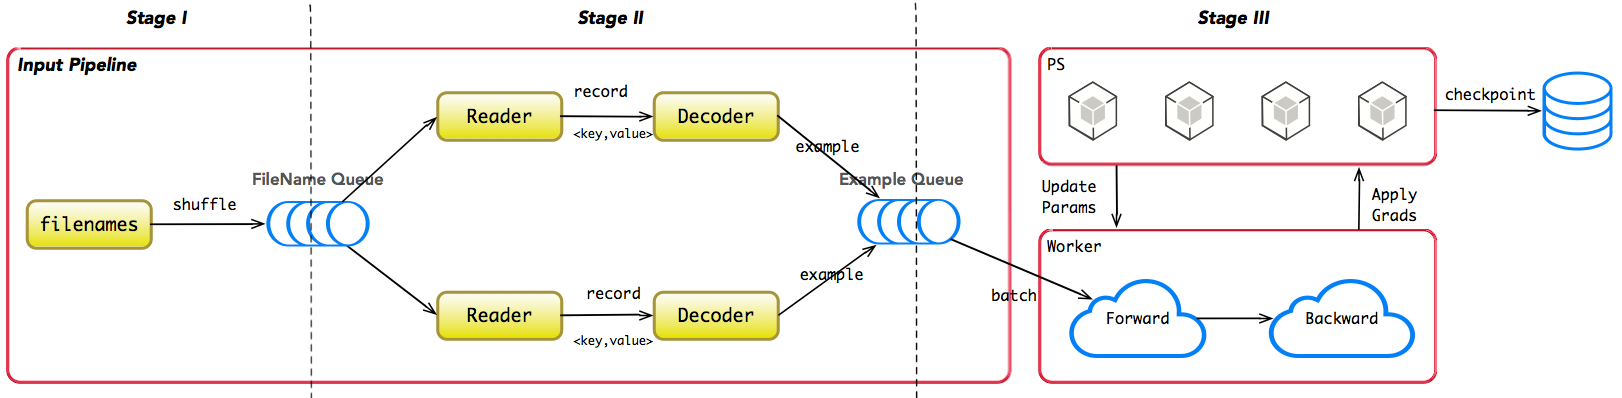
\includegraphics[width=0.9\textwidth]{figures/tf-input-pipeline.png}
\caption{模型训练工作流}
 \label{fig:tf-input-pipeline}
\end{figure}

\subsection{阶段1}

\code{string\_input\_producer}构造了一个\code{FIFOQueue}的队列,它是一个有状态的\ascii{OP}。根据\code{shuffle}选项,在每个\ascii{epoch}开始时,随机生成文件列表,并将其一同追加至队列之中。

\begin{figure}[!htbp]
\centering
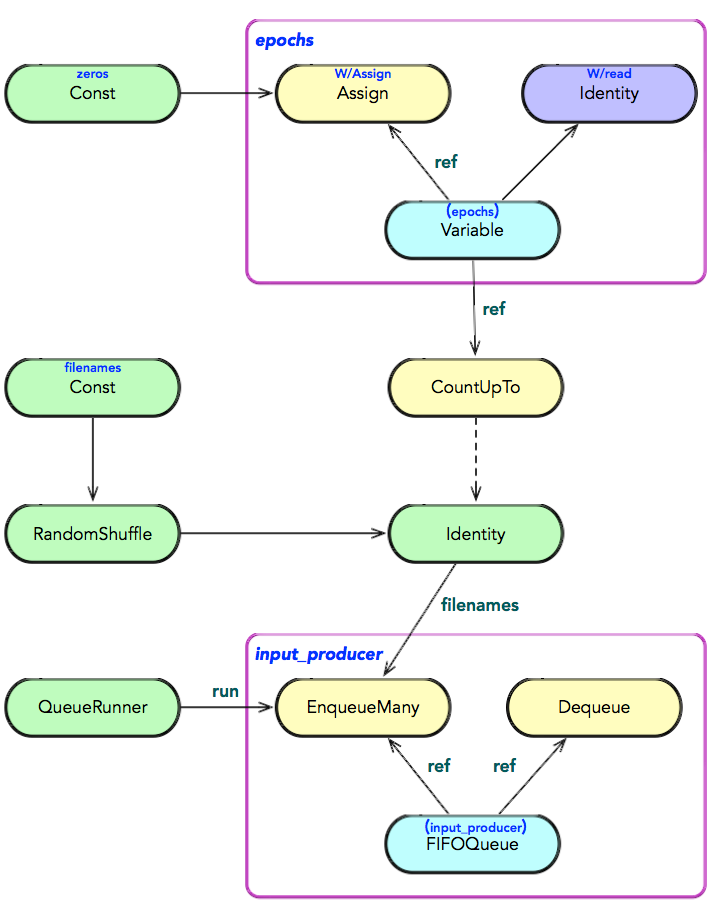
\includegraphics[width=0.7\textwidth]{figures/tf-input-pipeline-stage-1.png}
\caption{阶段1:模型训练工作流}
 \label{fig:tf-input-pipeline-stage-1}
\end{figure}

\subsubsection{随机化}

首先,执行名为\code{filenames}的\code{Const OP},再经过\code{RandomShuffle}将文件名称列表随机化。

\subsubsection{Epoch控制}

为了实现\ascii{epoch}的计数,实现巧妙地设计了一个名为\code{epochs}的本地变量。其中,本地变量仅对本进程的多轮Step之间共享数据,并且不会被训练子图实施更新。

在\code{Session.run}之前,系统会执行本地变量列表的初始化,将名为\code{epochs}的\code{Variable}实施零初始化。

\ascii{epoch}的计数功能由\code{CountUpTo}完成,它的工作原理类似于\ascii{C++}的\code{i++}。它持有\code{Variable}的引用,及其上限参数\code{limit}。每经过一轮\ascii{epoch},使其\code{Variable}自增1,直至达到\code{num\_epochs}数目。

其中,当\ascii{epoch}数到达\code{num\_epochs}时,\code{CountUpTo}将自动抛出\code{OutOfRangeError}异常。详细实现可以参考\code{CountUpToOp}的\ascii{Kernel}实现。

\begin{leftbar}
\begin{c++}
template <class T>
struct CountUpToOp : OpKernel {
  explicit CountUpToOp(OpKernelConstruction* ctxt)
    : OpKernel(ctxt) {
    OP_REQUIRES_OK(ctxt, ctxt->GetAttr("limit", &limit_));
  }

  void Compute(OpKernelContext* ctxt) override {
    T before_increment;
    {
      mutex_lock l(*ctxt->input_ref_mutex(0));
      
      // Fetch the old tensor
      Tensor tensor = ctxt->mutable_input(0, true);
      T* ptr = &tensor.scalar<T>()();      
      before_increment = *ptr;
      
      // throw OutOfRangeError if exceed limit
      if (*ptr >= limit_) {
        ctxt->SetStatus(errors::OutOfRange(
            "Reached limit of ", limit_));
        return;
      }
      // otherwise increase 1
      ++*ptr;
    }
    // Output if no error.
    Tensor* out_tensor;
    OP_REQUIRES_OK(ctxt, ctxt->allocate_output(
        "output", TensorShape({}), &out_tensor));
    out_tensor->scalar<T>()() = before_increment;
  }

private:
  T limit_;
};
\end{c++}
\end{leftbar}

\subsubsection{入队操作}

事实上,将文件名列表追加到队列中,执行的是\code{EnqueueMany},类似于\code{Assign}修改\code{Variable}的值,\code{EnqueueMany}也是一个有状态的\ascii{OP},它持有队列的句柄,直接完成队列的状态更新。

在此处,\code{EnqueueMany}将被\code{Session.run}执行,系统反向遍历,找到依赖的\code{Identity},发现控制依赖于\code{CountUpTo},此时会启动一次\ascii{epoch}计数,直至到达\code{num\_epoch}数目抛出\code{OutOfRangeError}异常。同时,\code{Identity}依赖于\code{RandomShuffle},以便得到随机化了的文件名列表。

\subsubsection{QueueRunner}

另外,在调用\code{tf.train.string\_input\_producer}时,将往计算图中注册一个特殊的\ascii{OP}:\code{QueueRunner},并且将其添加到\code{GraphKeys.QUEUE\_RUNNERS}集合中。并且,一个\code{QueueRunner}持有一个或多个\code{Enqueue, EnqueueMany}类型的\ascii{OP}。

\subsection{阶段2}

\code{Reader}从文件名队列中按照\ascii{FIFO}的顺序获取文件名,并按照文件名读取文件记录,成功后对该记录进行解码和预处理,将其转换为数据样本,最后将其追加至样本队列中。

\subsubsection{读取器}

事实上,实现构造了一个\code{ReaderRead}的\ascii{OP},它持有文件名队列的句柄,从队列中按照\ascii{FIFO}的顺序获取文件名。

因为文件的格式为\code{TFRecord},\code{ReaderRead}将委托调用\code{TFRecordReader}的\ascii{OP},执行文件的读取。最终,经过\code{ReaderRead}的运算,将得到一个序列化了的样本。

\subsubsection{解码器}

得到序列化了的样本后,将使用合适的解码器实施解码,从而得到一个期望的样本数据。可选地,可以对样本实施预处理,例如\code{reshape}等操作。

\subsubsection{入队操作}

得到样本数据后,将启动\code{QueueEnqueue}的运算,将样本追加至样本队列中去。其中,\code{QueueEnqueue}是一个有状态的\ascii{OP},它持有样本队列的句柄,直接完成队列的更新操作。

实施上,样本队列是一个\code{RandomShuffleQueue},使用出队操作实现随机采样。

\subsubsection{并发执行}

为了提高\ascii{IO}的吞吐率,可以启动多路并发的\code{Reader}与\code{Decoder}的工作流,并发地将样本追加至样本队列中去。其中,\code{RandomShuffleQueue}是线程安全的,支持并发的入队或出队操作。

\subsection{阶段3}

当数据样本累计至一个\code{batch\_size}时,训练/推理子图将取走该批次的样本数据,启动一次迭代计算(常称为一次\ascii{Step})。

\subsubsection{出队操作}

事实上,训练子图使用\code{DequeueMany}获取一个批次的样本数据。

\subsubsection{迭代执行}

一般地,一次迭代运行,包括两个基本过程:前向计算与反向梯度传递。\ascii{Worker}任务使用\ascii{PS}任务更新到本地的当前值,执行前向计算得到本次迭代的损失。

然后,根据本次迭代的损失,反向计算各个\ascii{Variable}的梯度,并更新到\ascii{PS}任务中;\ascii{PS}任务更新各个\code{Variable}的值,并将当前值广播到各个\ascii{Worker}任务上去。

\subsubsection{Checkpoint}

\ascii{PS}任务根据容错策略,周期性地实施\ascii{Checkpoint}。将当前所有\code{Variable}的数据,及其图的元数据,包括静态的图结构信息,持久化到外部存储设备上,以便后续恢复计算图,及其所有\code{Variable}的数据。

\subsection{Pipeline节拍}

例如,往\code{FIFOQueue}的队列中添加文件名称列表,此时调用\code{EnqueueMany}起始的子图计算,其中包括执行所依赖的\code{CountUpTo}。当\code{CountUpTo}达到\code{limit}上限时,将自动抛出\code{OutOfRangeError}异常。

扮演主程序的\code{QueueRunner},捕获\code{coord.join}重新抛出的\code{OutOfRangeError}异常,随后立即关闭相应的队列,并且退出该线程的执行。队列被关闭之后,入队操作将变为非法;而出队操作则依然合法,除非队列元素为空。

同样的道理,下游\ascii{OP}从队列(文件名队列)中出队元素,一旦该队列元素为空,则自动抛出\code{OutOfRangeError}异常。该阶段对应的\code{QueueRunner}将感知该异常的发生,然后捕获异常并关闭下游的队列(样本队列),退出线程的执行。

在\ascii{Pipeline}的最后阶段,\code{train\_op}从样本队列中出队批次训练样本时,队列为空,并且队列被关闭了,则抛出\code{OutOfRangeError}异常,最终停止整个训练任务。
